% !TeX TXS-program:compile = txs:///pdflatex/[--shell-escape]

\documentclass[9pt]{beamer}
\usetheme{Madrid}
\usecolortheme{beaver}
\usepackage{amsmath,amssymb,amsthm,asymptote,graphicx}
\usepackage{graphics}
% \usepackage{bisvslides}
\usepackage{arcs}
\graphicspath{{./images}}

\newcounter{problem}[section]

% \newenvironment{probslide}[3][]{%
%     \refstepcounter{problem}\begin{frame}[t]%
% 	{Problem \thesection.\theproblem 
%         \def\temp{#2}\ifx\temp\empty
%             %
%         \else
%             \ - \temp%
%         \fi}
%     {#3}}%
% 	{\end{frame}}

% \newenvironment{Example}[2][Example]
%     {This is an #1. You gave #2 as an argument. The rest will be bold: \bfseries}
%     {}
% \textbf{Problem~\theproblem. #1
% \newenvironment{bsmi}{\begin{CJK}{UTF8}{bsmi}}{\end{CJK}}

\title{Mixed Advanced Topics}
\subtitle{Mathcounts 21 - Session 4}
\author{Rohan D., Derrick L., Irene W.}
\institute{BISV Mathcounts Club 21}
\date{January 4, 2022}

%\maketitle
%~~~~~~~~~~~~~~~~~~~~~~~~~~~~~~~~~~~~~~~~~~~~~~~~~~~~~~~~~~~~~~~~~~~~~~~~~~~~~~
% Informations
%\title{TEMPLATE}

%\titlegraphic{assets/gkg.png} %change this to your preferred logo or image(the image is located on the top right corner).
%~~~~~~~~~~~~~~~~~~~~~~~~~~~~~~~~~~~~~~~~~~~~~~~~~~~~~~~~~~~~~~~~~~~~~~~~~~~~~~

\begin{document}

% Generate title page
\begin{frame}
    \titlepage        
\end{frame}
% \setbeamertemplate{footline}[miniframes Madrid]

\setcounter{section}{2}

\section{Intermediate Practice Problems}

\refstepcounter{problem}
\begin{frame}[t, fragile]{Problem \thesection.\theproblem}
    \begin{block}{}[2017 AMC 10B, \#13]
There are $20$ students participating in an after-school program offering classes in yoga, bridge, and painting. Each student must take at least one of these three classes, but may take two or all three. There are $10$ students taking yoga, $13$ taking bridge, and $9$ taking painting. There are $9$ students taking at least two classes. How many students are taking all three classes?
    
    \end{block}
\end{frame}


% Mass Point
\refstepcounter{problem}
\begin{frame}[t, fragile]{Problem \thesection.\theproblem}
    \begin{block}{}[Mathcounts 2015 State Sprint \#28]
In regular pentagon $ABCDE,$ point $M$ is the midpoint of side $AE,$ and segments
$AC$ and $BM$ intersect at point $Z.$ If $ZA = 3,$ what is the value of $AB?$ Express
your answer in simplest radical form.

    \end{block}
\end{frame}


% Counting
\refstepcounter{problem}
\begin{frame}[t, fragile]{Problem \thesection.\theproblem}
    \begin{block}{}[Mathcounts National 2018, Sprint \#7]
    Alice and Bob play a game that begins with flipping a fair coin twice. If the coin lands heads up on both flips,Bob wins. If the coin lands heads up on only one flip, Alice wins. If the coin lands tails up on both flips, they flip two more times, and this process continues until there is a winner. What is the probability that Bob wins the game? Express your answer as a common fraction.
    
    \end{block}
\end{frame}


% Probability
\refstepcounter{problem}
\begin{frame}[t, fragile]{Problem \thesection.\theproblem}
    \begin{block}{}[Mathcounts National 2018, Sprint \#10]
    What is the probability that a randomly chosen positive integer factor of 11,088 is not divisible by any perfect square greater than 1? Express your answer as a common fraction.
    
    \end{block}
\end{frame}


% 3D Geometry
\refstepcounter{problem}
\begin{frame}[t, fragile]{Problem \thesection.\theproblem}
    \begin{block}{}[BmMT 2019, \#19]
An ant sits on the circumference of the circular base of a party hat (a cone without a circular
base for the ant to walk on) of radius $2$ and height $\sqrt{5}$. If the ant wants to reach a point
diametrically opposite of its current location on the hat, what is the minimum possible distance
the ant needs to travel?


    \end{block}
    \begin{center}
        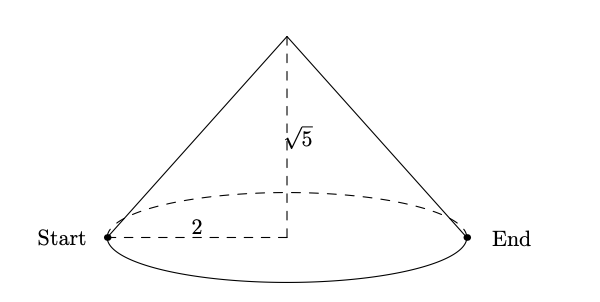
\includegraphics[scale=0.5]{bmmt2019_19_p}
    \end{center}
\end{frame}



\refstepcounter{problem}
\begin{frame}[t, fragile]{Problem \thesection.\theproblem}
    \begin{block}{}[Mathcounts National 2018, Sprint \#14]
    Jenny rolls four standard six-sided dice, each with faces numbered one through six.What is the probability that there is at least one pair of dice whose top faces sum to 12? Express your answer as a common fraction.
    
    \end{block}
\end{frame}


% Counting with symmetries
\refstepcounter{problem}
\begin{frame}[t, fragile]{Problem \thesection.\theproblem}
    \begin{block}{}[Mathcounts National 2018, Sprint \#15]
    The faces of two cubes are painted so that the colors of the six faces on each cube are red,orange, yellow, green, blue and violet, in some random order. What is the probability that the two cubes can be rotated so that their colorings are identical? Express your answer as a common fraction.
    
    \end{block}
\end{frame}


% Coordinate Geometry
\refstepcounter{problem}
\begin{frame}[t, fragile]{Problem \thesection.\theproblem}
    \begin{block}{}[Mathcounts National 2018, Sprint \#11]
    The graph of the line $ 2x+3y=8 $ intersects the $ x $-axis at $ A $ and intersects the $ y $-axis at $ B $. Points $ A,B $ and $ O(0,0) $ form right triangle $ ABO $. If triangle $ ABO $ is dilated about the origin by a scale factor of $ -\frac{3}{4} $, what is the area of dilated triangle $ A'B'O' $?
    
    \end{block}
\end{frame}


% 3D Geometry

\refstepcounter{problem}
\begin{frame}[t, fragile]{Problem \thesection.\theproblem}
    \begin{block}{}[Mathcounts National 2018, Sprint \#16]
    The bases of the right hexagonal prism shown are regular hexagons with sides of length 4 inches. Space diagonals $ AD' $ and $ CF' $ intersect at a right angle. What is the length of edge $ EE' $? Express your answer in simplest radical form.

    
    \end{block}
    \begin{center}
        \begin{asy}
        import three;        
        currentprojection=orthographic(3, -50, 20);

        unitsize(0.5cm);
        real s = 4;

        pair A, A1, B, B1, C, C1, D, D1, E, E1, F, F1;

        F = (0,0);
        E = (s, 0);
        A = rotate(120, F)*E;
        D = rotate(-120, E)*F;
        C = rotate(-120, D)*E;
        B = rotate(-120, C)*D;

        draw((F.x, F.y, 0)--(E.x, E.y, 0)--(D.x, D.y, 0)--(C.x, C.y, 0)--(B.x, B.y, 0)--(A.x, A.y, 0)--cycle);
        draw((F.x, F.y, -s)--(E.x, E.y, -s)--(D.x, D.y, -s)--(C.x, C.y, -s)--(B.x, B.y, -s)--(A.x, A.y, -s)--cycle);
        draw((F.x, F.y, 0)--(F.x, F.y, -s)^^(E.x, E.y, 0)--(E.x, E.y, -s)^^(D.x, D.y, 0)--(D.x, D.y, -s)^^(C.x, C.y, 0)--(C.x, C.y, -s)^^(B.x, B.y, 0)--(B.x, B.y, -s)^^(A.x, A.y, 0)--(A.x, A.y, -s));

        draw((A.x, A.y, 0)--(D.x, D.y, -s)^^(C.x, C.y, 0)--(F.x, F.y, -s), dashed);

        label("$A$", (A.x, A.y, 0), N);
        label("$B$", (B.x, B.y, 0), N);
        label("$C$", (C.x, C.y, 0), N);
        label("$D$", (D.x, D.y, 0), N);
        label("$E$", (E.x, E.y, 0), N);
        label("$F$", (F.x, F.y, 0), N);

        label("$A'$", (A.x, A.y, -s), S);
        label("$B'$", (B.x, B.y, -s), S);
        label("$C'$", (C.x, C.y, -s), S);
        label("$D'$", (D.x, D.y, -s), S);
        label("$E'$", (E.x, E.y, -s), S);
        label("$F'$", (F.x, F.y, -s), S);

        \end{asy}
    \end{center}
    

\end{frame}


% Counting
\refstepcounter{problem}
\begin{frame}[t, fragile]{Problem \thesection.\theproblem}
    \begin{block}{}[Mathcounts National 2018, Sprint \#17]
    In a card game, Nora draws cards at random, without replacement,from a deck of 21 cards. Twenty of the cards are numbered 1 through 20, and the other card is marked ``Joker.'' Nora keeps all of the cards she draws before she draws the Joker. What is the probability that the cards Nora keeps include exactly four prime-numbered cards? Express your answer as a common fraction.
    
    \end{block}
\end{frame}


% Counting and Number Theory
\refstepcounter{problem}
\begin{frame}[t, fragile]{Problem \thesection.\theproblem}
    \begin{block}{}[Mathcounts National 2018, Sprint \#18]
    How many assignments of digits $ A, B, C $ and $ D $ exist such that the four-digit numbers $ ABCD_6 $ and $ ABCD_{10} $ are both divisible by 5?
    
    \end{block}
\end{frame}


\refstepcounter{problem}
\begin{frame}[t, fragile]{Problem \thesection.\theproblem}
    \begin{block}{}[Mathcounts National 2018, Sprint \#19]
    In the figure, $ ABCD $ is a square with area $ 1024 \text{ cm}^2 $. $ P $ is the midpoint of side $ CD $. $ Q $ is the midpoint of segment $ BP $. $ R $ is the midpoint of segment $ AQ $. $ S $ is the midpoint of segment $ DR $. $ T $ is the midpoint of segment $ CS $. $ T $ is also the intersection of segments $ BP $ and $ CS $. What is the area of quadrilateral $ QRST $?
    
    \end{block}
    \begin{center}
        \begin{asy}
            unitsize(0.75cm);
            real s = 5;
            pair A, B, C, D, P, Q, R, S, T;

            A = (s,s);
            B = (0,s);
            C = (0,0);
            D = (s,0);

            P = (C+D)/2;
            Q = (B+P)/2;
            R = (A+Q)/2;
            S = (D+R)/2;
            T = (C+S)/2;

            draw(A--B--C--D--cycle);
            draw(B--P^^A--Q^^D--R^^C--S);

            label("$A$", A, NE);
            label("$B$", B, NW);
            label("$C$", C, SW);
            label("$D$", D, SE);
            label("$P$", P, SE);
            label("$Q$", Q, SW);
            label("$R$", R, NW);
            label("$S$", S, NE);
            label("$T$", T, N);

        \end{asy}
    \end{center}

\end{frame}


% Counting Paths with Casework
\refstepcounter{problem}
\begin{frame}[t, fragile]{Problem \thesection.\theproblem}
    \begin{block}{}[Mathcounts National 2018, Sprint \#20]
    Vanessa tosses a fair coin eight times. If the coin lands heads up, she steps 1 meter west. If the coin lands tails up, she steps 1 meter north. What is the probability that Vanessa ends a distance of at most 6 meters away from her starting position? Express your answer as a common fraction.
    
    \end{block}
\end{frame}

%--------------



% Geometric Probability
\refstepcounter{problem}
\begin{frame}[t, fragile]{Problem \thesection.\theproblem}
    \begin{block}{}[Mathcounts National 2018, Target \#6]
    Micaela randomly chooses a real number $ w $ between -20 and 20. What is the probability that the graphs of $ x -|y| = w $ and $ x^2 + y^2 = 50 $ intersect at exactly two points? Express your answer as a decimal to the nearest hundredth.
    
    \end{block}
\end{frame}

%--------------



\refstepcounter{problem}
\begin{frame}[t, fragile]{Problem \thesection.\theproblem}
    \begin{block}{}
    A circle with center $O$ has radius 8 units and circle $P$ has radius 2 units. The circles are externally tangent to each other at point $Q$. Segment $TS$ is the common external tangent to circle $O$ and circle $P$ at points $T$ and $S$, respectively. What is the length of segment $OS$? Express your answer in simplest radical form.
	
    \end{block}
\end{frame}




\refstepcounter{problem}
\begin{frame}[t, fragile]{Problem \thesection.\theproblem}
    \begin{block}{}[Mathcounts National 2017, Sprint \#14]
    Philippa stands on the shaded square of the 8-by-8 checkerboard
shown. She moves to one of the four adjacent squares sharing
an edge with her starting square, with each of the four squares
equally likely to be chosen. She then makes two more moves
to adjacent squares in the same way. Given any square $ S $, let $ P(S) $ be the
probability that Philippa lands on that square after her third move. What is the
greatest possible value of $ P(S) $? Express your answer as a common fraction.

    \end{block}
    \begin{center}
        \begin{asy}
            unitsize(0.5cm);
            
            pair pos;
            pos = (3,4);
            for (int i = 0; i < 9; ++i) {
                draw((i,0)--(i,8)^^(0,i)--(8,i));
            }
            fill(pos--(pos.x + 1,pos.y)--(pos.x+1,pos.y+1)--(pos.x,pos.y+1)--cycle, grey);
        \end{asy}
    \end{center}
	
\end{frame}


\refstepcounter{problem}
\begin{frame}[t, fragile]{Problem \thesection.\theproblem}
    \begin{block}{}[Mathcounts National 2017, Sprint \#19]
    Sam creates a six-digit positive integer by writing the digit 7 in the
hundred-thousands place, and then tossing a fair coin five times. If the coin
comes up heads, he writes a 7 for the next digit; if the coin comes up tails,
he writes a 0 for the next digit. What is the probability that Sam’s number is
divisible by 77? Express your answer as a common fraction.
	
    \end{block}
\end{frame}


\refstepcounter{problem}
\begin{frame}[t, fragile]{Problem \thesection.\theproblem}
    \begin{block}{}[Mathcounts National 2017, Sprint \#22]
    How many ways are there to fill in each empty square in the diagram below with
a positive integer so that no integer appears more than once in the diagram, and
every integer in the diagram is less than each integer to its right?

    \end{block}
    \begin{center}
        \begin{asy}
            unitsize(1cm);
            
            for (int i = 0; i < 8; ++i) {
                if (i != 2 && i != 5) {
                    draw((i,0)--(i+1,0)--(i+1,1)--(i,1)--cycle);
                } else {
                    draw((i,-0.5)--(i+1,-0.5)--(i+1,1.5)--(i,1.5)--cycle^^(i,0.5)--(i+1,0.5));
                }
            }
            label("$12$", (7.5,0.5));
        \end{asy}
    \end{center}
	
\end{frame}


\refstepcounter{problem}
\begin{frame}[t, fragile]{Problem \thesection.\theproblem}
    \begin{block}{}[Mathcounts National 2017, Sprint \#23]
    What is the total surface area of the largest regular tetrahedron that can be
    inscribed inside of a cube of edge length 1 cm? Express your answer in simplest
    radical form.
	
    \end{block}
\end{frame}



\refstepcounter{problem}
\begin{frame}[t, fragile]{Problem \thesection.\theproblem}
    \begin{block}{}[Mathcounts National 2017, Sprint \#24]
    Penny flips three fair coins into a box with two compartments. Each
compartment is equally likely to receive each of the coins. What is the
probability that either of the compartments has at least two coins that landed
heads? Express your answer as a common fraction.
	
    \end{block}
\end{frame}



\refstepcounter{problem}
\begin{frame}[t, fragile]{Problem \thesection.\theproblem}
    \begin{block}{}[Mathcounts National 2017, Sprint \#30]
    In the figure shown, two lines intersect at a right angle, and two
    semicircles are drawn so that each semicircle has its diameter on
    one line and is tangent to the other line. The larger semicircle has
    radius 1. The smaller semicircle intersects the larger semicircle,
    dividing the larger semicircular arc in the ratio 1:5. What is the
    radius of the smaller semicircle? Express your answer in simplest
    radical form.
    
    \end{block}
    \begin{center}
        \begin{asy}
            unitsize(2cm);
            import cse5;
            pair O1, O2, T;
    
            real r1 = 1, r2 = 2 - sqrt(3);
    
            O1 = (0,r1);
            O2 = (r2,0);
            draw((2.5,0)--(0,0)--(0,2.5));
    
            draw(arc(O1, r1, -90, 90));
            draw(arc(O2, r2, 0, 180));
    
        \end{asy}
        \end{center}
        
    \end{frame}



\refstepcounter{problem}
\begin{frame}[t, fragile]{Problem \thesection.\theproblem}
    \begin{block}{} [Mathcounts National 2017, Target \#6]
Two congruent squares with side length 4 have equilateral triangles constructed
in them as shown. In one square, one side of the equilateral triangle is a side
of the square. In the other square, the equilateral triangle has one vertex at a
vertex of the square and its other two vertices are on the sides of the square. The
absolute difference of the areas of the two triangles can be expressed in simplest
radical form as $a\sqrt{b} + c$. What is the value of $a + b + c$?

    \end{block}
    \begin{center}
        \begin{asy}
        unitsize(2cm);
        pair A, B, C, D;
        pair P1, P2, P3;
        
        picture pic1, pic2;
        
        A = (-2,0);
        B = (-2,2);
        C = (0,2);
        D = (0,0);
        
        P1 = rotate(-60)*A;
        P2 = extension(rotate(-15)*A, D, A, B);
        P3 = extension(rotate(-75)*A, D, B, C);
        
        draw(pic1, A--B--C--D--cycle^^D--P1--A);
        label(pic1, "$4$", A--D, S);
        label(pic1, "$4$", A--B, W);
        
        draw(pic2, A--B--C--D--cycle^^D--P2--P3--cycle);
        label(pic2, "$4$", A--D, S);
        label(pic2, "$4$", D--C, E);
    
        add(shift(2.5*right)*pic2);
    
        add(pic1);
        \end{asy}
    \end{center}
        
    \end{frame}


\refstepcounter{problem}
\begin{frame}[t, fragile]{Problem \thesection.\theproblem}
    \begin{block}{}[Mathcounts National 2017, Target \#3]
    There are a hundred competitors at the National Debating Contest, two from
each of the 50 states. In how many ways can five finalists be chosen if no state
may have more than one finalist?
	
    \end{block}
\end{frame}


\refstepcounter{problem}
\begin{frame}[t, fragile]{Problem \thesection.\theproblem}
    \begin{block}{}[Mathcounts National 2017, Target \#4]
    Rays $AC$ and $AE$ intersect circle $O$ at $B$ and $D$, respectively. Segment $DE$ is a
diameter of circle $O$ and $AB = \frac{1}{2}DE$. If the measure of $ \angle BAD$ is 24 degrees, what is the degree measure of $ \angle COE$ ?

    \end{block}
    \begin{center}
        \begin{asy}
        unitsize(2cm);
        pair O, A, B, C, Cp, D, E;
        
        O = (0,0);
        E = (1,0);
        D = (-1,0);
        C = rotate(72)*E;
        B = rotate(-24)*D;
        
        Cp = -0.5*B+1.5*C;
        
        A = extension(C, B, E, D);
        
        draw(circle(O, 1));
        dot(C);
        dot(B);
        dot(D);
        dot(E);
        dot(O);
        dot(A);
        draw(A--Cp, EndArrow);
        draw(A--(1.5,0), EndArrow);
        draw(O--C);
        
        label("$O$", O, S);
        label("$D$", D, SW);
        label("$E$", E, SE);
        label("$C$", C, NE);
        label("$B$", B, NW);
        label("$A$", A, S);
        
        \end{asy}
    \end{center}
        
    \end{frame}



\refstepcounter{problem}
\begin{frame}[t, fragile]{Problem \thesection.\theproblem}
    \begin{block}{}[Mathcounts National 2016, Sprint \#21]
    Manny has two red socks, two white socks, and two blue socks. He plans to choose two socks at random to wear today, two of the remaining socks to wear tomorrow, and will wear the last two remaining socks the next day. What is the probability that on all three days, Manny wears two different colored socks? Express your answer as a common fraction.
	
    \end{block}
\end{frame}


\refstepcounter{problem}
\begin{frame}[t, fragile]{Problem \thesection.\theproblem}
    \begin{block}{}[Mathcounts National 2016, Sprint \#30]
    In isoceles triangle $ABC$, with base $BC$ of length 23 cm, points $P$ and $Q$ are chosen such that $BP = CQ = 9$ cm. If segments $AP$ and $AQ$ trisect angle $BAC$, what is the perimeter of $\triangle ABC$? 
	
    \end{block}
\end{frame}


\refstepcounter{problem}
\begin{frame}[t, fragile]{Problem \thesection.\theproblem}
    \begin{block}{}[Mathcounts National 2018, Target \#8]
    Shane cuts out a paper circle of radius 7 cm. He then draws two perpendicular chords, as shown, with one a distance of 1 cm from the center and the other 3 cm from the center. Next, Shane folds the bottom of the circle up along the first chord and then folds the left side of the folded circle to the right along the second chord. If the folded arcs intersect at a point P, as shown, what is the distance from the vertex of the right angle formed by the folds to P? Express your answer in simplest radical form.

    \end{block}
    \begin{center}
        \begin{asy}
            unitsize(0.30cm);

            picture p1, p2;
            pair O, O1, O2, A1, A2, B1, B2, P, Q, M;
            pair ip[];

            path c, a1, a2;

            O = (0, 0);
            O1 = (-6, 0);
            O2 = (0, -2);

            M = (-3,-1);

            c = circle(O, 7);

            ip = intersectionpoints(c, (-3,-7)--(-3,7));
            A1 = ip[0];
            B1 = ip[1];

            ip = intersectionpoints(c, (-7,-1)--(7,-1));
            A2 = ip[0];
            B2 = ip[1];

            Q = intersectionpoints(circle(O1, 7), M--B2)[0];

            a1 = arc(O1, Q, A1);

            P = intersectionpoints(a1,circle(O2, 7))[0];
            a2 = arc(O2, B2, P);

            draw(p1, c);
            dot(p1, O);
            // dot(p1, A1, red);
            // dot(p1, A2, blue);

            draw(p1, A1--B1^^A2--B2, dashed);

            draw(p2, arc(O, B2, A1)--M--cycle^^a1^^a2);
            draw(p2, M--P, dashed);
            dot(p2, P);
            dot(p2, O);

            label(p2, "$P$", P, NE);
            label(p2, "?", M--P, SE);

            add(p1);
            add(shift(15*right)*p2);
        \end{asy}
    \end{center}
    
\end{frame}

%--------------

\newpage

\section{Challenge Problems}
\refstepcounter{problem}
\begin{frame}[t, fragile]{Problem \thesection.\theproblem}
    \begin{block}{}[2001 AIME I, \#7]
    Triangle $ABC$ has $AB=21$, $AC=22$ and $BC=20$. Points $D$ and $E$ are located on $\overline{AB}$ and $\overline{AC}$, respectively, such that $\overline{DE}$ is parallel to $\overline{BC}$ and contains the center of the inscribed circle of triangle $ABC$. Then $DE=m/n$, where $m$ and $n$ are relatively prime positive integers. Find $m+n$.	

    \textit{Hint: The incenter is at the intersection of angle bisectors.}

    \end{block}
\end{frame}


\refstepcounter{problem}
\begin{frame}[t, fragile]{Problem \thesection.\theproblem}
    \begin{block}{}[1998 AIME, \# 9]
    Two mathematicians take a morning coffee break each day. They arrive at the cafeteria independently, at random times between 9 a.m. and 10 a.m., and stay for exactly $m$ minutes. The probability that either one arrives while the other is in the cafeteria is $40 \%,$ and $m = a - b\sqrt {c},$ where $a, b,$ and $c$ are positive integers, and $c$ is not divisible by the square of any prime. Find $a + b + c.$
	
    \end{block}
\end{frame}


\refstepcounter{problem}
\begin{frame}[t, fragile]{Problem \thesection.\theproblem}
    \begin{block}{}[HMMT 2003]
    Find the smallest $n$ such that $n!$ ends in 290 zeroes.
	
    \end{block}
\end{frame}



\end{document}
